\documentclass[]{mtprarprt}

\title{Masteroppgaven min <3}
\subtitle{Leveraging Large Language Models to Achieve Semantic Reasoning in Robots}
\author{Elias Helle Kalland}

\addbibresource{references.bib} 

\usepackage{layout}
\usepackage{algorithm}
\usepackage{algpseudocode}
\usepackage{listings}
\usepackage{amsthm}
\usepackage{svg}
\usepackage{multirow}
\usepackage{graphicx}

\lstset{captionpos=b}

\theoremstyle{definition}
\newtheorem{example}{Example}[section]

\begin{document}

\maketitle

\frontmatter

\chapter{Preface}
\chapter{Summary}
\tableofcontents
\listoffigures
\listoftables
\lstlistoflistings

\mainmatter
\chapter{}
\chapter{Preliminaries}

\section{Behaviour trees}
A behaviour tree (BT) is a tool for defining and organising decision-making processes and actions for a robot. It consists of nodes connected in a "tree" structure. Nodes are connected through parent and child nodes, where the root node is the only node without a parent. Nodes are divided into control flow nodes and execution nodes. There are four types of control flow nodes, namely Sequence, Fallback, Parallel and Decorator, and two types of execution nodes, Action and Condition.

The BT is executed from the root node by a tick that is sent to its child nodes from left to right. The child node returns Running, Success or Failure to its parent based on the current state of the child. A node can only be executed if it receives a tick.

A Sequence node with N children will tick all its children until one returns Failure. If all children return Success, the Sequence node will return Success to its own parent. The Fallback node is the same, except that it will tick its children until a child returns Success. If all children return Failure, the Fallback node will return Failure to its own parent.
The Parallel node ticks its $N$ children and returns Success if $M$ children return Success, Failure if $N-M+1$ children return Failure and Running otherwise. $M$ is a user-specified number.
Finally, the Decorator node is a node that modifies the return status of its child, based on the users need. It ticks its child based on a user-specified rule and is therefore customised based on what application the BT is used for.

The two execution nodes, Action and Condition, perform an action or check if a condition holds, respectively. A Condition node never returns Running \cite[p. 5-9]{colledanchise_behavior_2018}.

\textcolor{red}{figur av de forskjellige nodene}

% \subsection{BT with ROS 2}
% \textcolor{red}{Mye kopi fra The Construct! Må skrives om.}
% \subsubsection{Part 1}
% \subsubsection{Part 2}
% \subsubsection{Part 3}
% The action defined by a BT node is called a callback. A ROS node communicates with a robot and receives feedback from it. The feedback is processed and the state is sent to the BT node. The return is then sent to the Root. When designing a BT, you don't have to know the details of the ROS node, only the behaviour of the node.
% ROS part of the program contains nodes that performs different actions on the robot. These actions are available by the BT node actions.

% For a Sequence node, it ticks its children one at a time. If it returns true it ticks next. If the second returns Running, the parent node will tick again in the next frequency. The state of the first child node is remembered, so it will skip this now. If the Running node now returns Success, it moves on to the next node an so forth.

% XML files are used to model a BT's logical structure.

% Reactive Sequential node is an asynchronous node. When a child returns Failure or Running it will restart.

% The BT.CPP framework executes nodes concurrently. The tree execution engine is single-threaded, and the tick() methods are always executed sequentially. That means if one thick() is blocked, the entire execution is blocked. An action that takes a while to execute should therefore return Running.

% A Sequence star node has memory. When a children return Success, it is remembered and will not be checked again. Assume four actions A, B, C, D. Actions A and B are SUCCESS, but C is FAILURE, so the next tick will start from C (A and B are memorized).

% A Blackboard is a map container that stores key-value pairs. Values between nodes flow through the blackboard. A BT node can have an input port which reads an entry from the blackboard, while an output port can write into an entry on the blackboard. It is like an interface to the memory.

% \cite{auryn_robotics_about_2024}

\section{The Planning Domain Definition Language}
The Planning Domain Definition Language (PDDL) is a declarative language used to standardise automated planning problems. 

\cite{ghallab_pddl_1998}
\cite{alaboud_getting_2024}

\section{PlanSys2}

\section{Forward-Chaining Partial-Order Planning}

\cite{martin_plansys2_2021}
\chapter{System description}
This chapter covers the design and implementation of SemReBot2, a system architecture that enables a robot to gain semantic knowledge in natural language. It begins with a brief overview of the architecture before describing each module, including the simulation environment. The chapter ends with a deeper study of the modules and the data pipeline. See Appendix \textcolor{red}{X} for a video demo\footnote{As of April 24th 2024, the software packages used in SemReBot2 is migrating to Ubuntu 24.04. This creates dependency issues related to the simulation environment and graphical user interface\cite{stinkyelias_source_2024}. Therefore, the video demo is showing a terminal-like simulation environment instead of a 3D world.}.

SemReBot2 is specialized in a pick-and-place scenario of pallets in a simulated warehouse. The goal is to allow humans interfere with robots by using their voice only, which makes robots available for everyone that can speak. 

\section{SemReBot2 overview}
An overview of the SemReBot2 pipeline is shown in Figure \ref{fig:semrebot2_overview}. Based on human speech, SemReBot2 translates this speech into suitable actions that a robot can perform. SemReBot2 inputs natural language speech, $u_{s}$, and transforms it to natural language text, $u_{t}$, with ASR. An LLM generates PDDL problem instances $\mathbf{P}_{i}$, predicates $\mathbf{P}_{p}$ and goals $\mathbf{P}_{g}$, passed to PlanSys2 for evaluation. An AI planner within PlanSys2 generates a plan $\mathbf{P}_{plan}$ with corresponding actions $\mathbf{a}$ that a robot can execute in the physical world.

\begin{figure}[h]
    \centering
    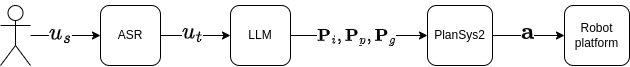
\includegraphics[width=\textwidth]{figures/overview_semrebot2.png}
    \caption[SemReBot2 overview]{Overview of SemReBot2 pipeline. There are no feedback loops in the pipeline.}
    \label{fig:semrebot2_overview}
\end{figure}

SemReBot2 leverages three main open source projects wrapped in ROS 2 to function: OpenAI's Whisper ASR model for speech-to-text tasks, MistralAI's Mistral 7B Instruct LLM for semantic reasoning, and PlanSys2, a PDDL-based planning system implemented in ROS 2.

\section{SemReBot2 modules}
SemReBot2 uses ROS 2 to combine the different components to run on a robotics platform.

\subsection{Automatic speech recognition module}
The first module in the data pipeline is the ASR module. The ASR module is the only module that directly interferes with a human by converting speech to text. The conversion is done by the large Whisper model. Whisper can be combined with ROS 2 through Hugging Face's transformers library in Python which also allows the user to load the model to a GPU with flash attention. The loading of the model with flash attention decreases the inference time (see Section \ref{sec:Whisper_experiments}) which we count as an important metric in a real-time robotics system.

In SemReBot2, automatic speech recognition is handled by the ROS 2 lifecycle node \newline\verb|whisper_lifecycle_node|. Figure \ref{fig:whisper_lifecycle} shows a simplified state diagram. Choosing it as a lifecycle node allows a fail-safe mechanism in case memory has to be freed or reallocated during runtime. It is also convenient during testing to isolate modules with managed state transitions.

\begin{figure}[h]
    \centering
    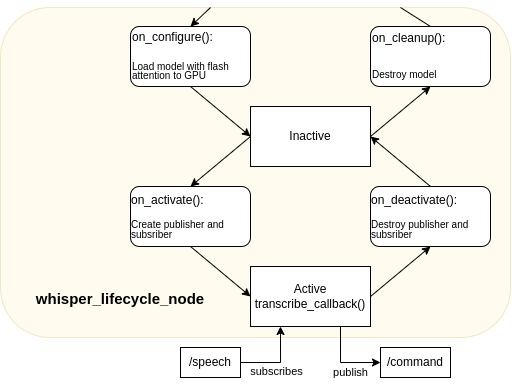
\includegraphics[width=0.8\textwidth]{figures/whisper_lifecycle.png}
    \caption[Whisper lifecycle node]{A simple state diagram of Whisper lifecycle node.}
    \label{fig:whisper_lifecycle}
\end{figure}

Upon activation, Whisper have been loaded to a GPU and the node is subscribing to the topic \verb|/speech|. Once a message is received, the \verb|transcribe_callback| method is called and the incoming audio $u_{s}$ is transcribed before it publishes $u_{t}$ as a \verb|std_msgs/msg/String| on the \verb|/command| topic. Until a new message is received, our Whisper node is on standby.

\subsection{Large language model module}
The large language model module boasts the same skeleton design as \verb|whisper_lifecycle_node|. It is a managed lifecycle node running Mistral 7B model in 4-bit quantized size. Again, Hugging Face's transformers library lets us load the model in a Python script and use it with ROS 2. The \verb|BitsAndBytesConfig| class allows us to load the model in 4-bit, which greatly reduces memory allocation (although at the cost of performance) compared to the full precision model.

\begin{figure}[ht]
    \centering
    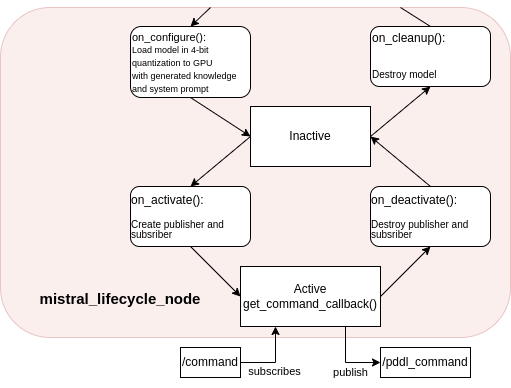
\includegraphics[width=0.8\textwidth]{figures/mistral_lifecycle.png}
    \caption[Mistral lifecycle node]{A simple state diagram of the Mistral lifecycle node.}
    \label{fig:mistral_lifecycle}
\end{figure}

When transitioning \verb|mistral_lifecycle_node| to a configured state, Mistral is loaded to the GPU with generated knowledge and a system prompt. The generated knowledge and system prompt is necessary in order to instruct Mistral to respond to commands in the desired format. The system prompt explains that Mistral is running on an AGV forklift as a "PDDL assistant". It also contains the necessary info from \verb|domain.pddl| such as the different types that is allowed and the possible predicates. Functions and actions are excluded, as they have no value for the language model.
Generated knowledge contains instances and predicates that are true at all times. That is, for example, the robot exists and the zones inside the warehouse have shelves or a charging station.

When the node's callback function is called, Mistral is few-shot prompted with ten examples to guide Mistral to answer in a certain way. A shot is designed to tell Mistral "given \textit{this} domain and command, output in \textit{this} format".

\begin{figure}[ht]
    \centering
    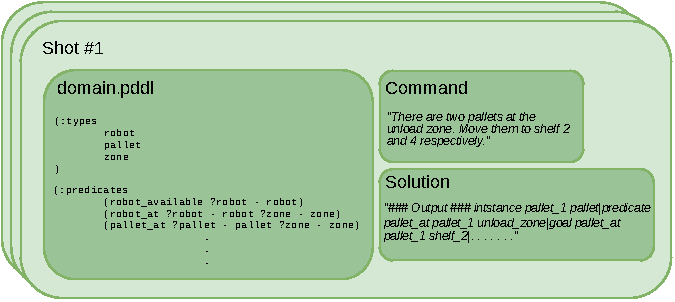
\includegraphics[width=\textwidth]{figures/few-shot_prompting.pdf}
    \caption[Few-shot prompting]{An example shot prompted to Mistral with the solution output, given a domain and command.}
    \label{fig:few_shot_prompt_mistral}
\end{figure}

The output format is designed in such a way that it can be passed to PlanSys2's client API (see Section \ref{ssec:semrebot2_task_controller}) with simple string parsing. The output format always begin with a prompt guard \verb|### Output ###| and ends with an end token "|". In this manner, any tokens generated by Mistral preceding the prompt guard and following the final end token can be discarded before passed to PlanSys2's client API by publishing a \verb|std_msgs/msg/String| to the \verb|/pddl_command| topic.

To keep the input memory at the same size as commands are given to Mistral, the previous command and output is discarded. The system prompt, generated knowledge, and the ten shots are all passed to the model for every inference call, which makes the allocated memory nearly steady.

\subsection{Task controller}\label{ssec:semrebot2_task_controller}
SemReBot2 interacts with PlanSys2 by running a node \verb|task_controller| as a client application to PlanSys2. With PlanSys2's client API, the \verb|task_controller| can interact with the \verb|Executor|, \verb|Planner|, \verb|Domain Expert| and \verb|Problem Expert| in PlanSys2 through shared pointers.

The Task controller receives the same generated knowledge as Mistral, and by initialization, it sends the generated knowledge including function values of robot speed, battery level and distances between zones to the \verb|Problem Expert|.

The node's callback function is called once a message on the topic \verb|/pddl_command| is published. This message is parsed and additional instances and predicates, as well as one or more goals, are sent to the \verb|Problem Expert|. Further, Task controller invokes the \verb|Problem Expert| and \verb|Domain Expert| to redirect the problem and domain to the \verb|Planner|, which creates a plan with the POPF plugin. If the plan from the \verb|Planner| is valid, Task controller invokes the \verb|Executor| to execute the plan by first building the BT trees necessary and then tick each BT node in correct order.

\begin{algorithm}\label{alg:task_controller}
\caption{Task Controller Node}
    \begin{algorithmic}[1]
        \State Add generated knowledge to problem\_expert
        \Procedure{task\_callback}{message}
            \For{parsed instance, predicate, goal \textbf{in} message}
                \State Add instance, predicate, goal to problem\_expert
            \EndFor
            \State domain := getDomain()
            \State problem := getProblem()
            \State plan := getPlan(domain, problem)
            \If{plan has value}
                \State Execute plan
            \EndIf
        \EndProcedure
    \end{algorithmic}
\end{algorithm}

\subsection{Custom behavior tree nodes}\label{ssec:custom_behavior_tree_nodes}
BT nodes represent the logic of robotic actions. We created six custom BT action nodes to simulate the necessary actions to pick up and place one or more pallets. The custom BT nodes are \verb|ApproachPallet|, \verb|LeavePallet|, \verb|LowerFork|, \verb|RaiseFork|, \verb|Navigate| and \verb|Recharge|, which can be combined into three BTs \verb|Navigate|, \verb|Transport| and \verb|Recharge|, that the BT builder can combine according to the provided plan from POPF.

Using the custom \verb|Navigate| BT node as an example, it is responsible for sending goal poses to Nav2's \verb|NavigateToPose| action based on a plan. SemReBot2 launches a ROS 2 node \newline\verb|navigate_cmd| which is an instance of PlanSys2's BTAction, which again is a BT action node. \verb|navigate_cmd| include parameters such as the waypoints in the warehouse and the XML schema of the \verb|Navigate| BT node.

\begin{lstlisting}[language=XML, caption=The custom BT node Navigate, label=lst:navigate_xml]
<root BTCPP_format="4" main_tree_to_execute = "MainTree">
    <BehaviorTree ID="MainTree">
        <Sequence name="root_sequence">
            <Navigate name="navigate" goal="{arg2}"/>
        </Sequence>
    </BehaviorTree>
</root>
\end{lstlisting}

When the BTAction node \verb|navigate_cmd| is activated, it creates the BT from the XML schema, Listing \ref{lst:navigate_xml}, and initialises a blackboard with ports including a shared pointer to a ROS 2 node and a goal pose. The goal pose is inserted to the blackboard by the Executor's BT builder in PlanSys2 and uses the \verb|?to-zone| parameter from the \verb|navigate| durative action in the PDDL plan (not to be mistaken by the \verb|Navigate| BT node or \verb|navigate_cmd| ROS node.

\begin{lstlisting}[caption={The PDDL action navigate's parameters}, label=lst:navigate_pddl]
(:durative-action navigate
    :parameters (?robot - robot ?from_zone - zone ?to_zone - zone)
\end{lstlisting}

When our custom BT node \verb|Navigate| is constructed, it retrieves the shared pointer to the ROS node \verb|navigate_cmd| and the goal from the PDDL plan from the blackboard. The shared pointer allows the \verb|Navigate| BT node to access the ROS parameters, which include the waypoint coordinates. When the \verb|Navigate| BT node is ticked, it checks the value in the key-value pair \verb|goal| in the blackboard and sends the corresponding coordinate as a goal to the \verb|NavigateToPose| action server, which is a part of the Nav2 navigation stack.

\subsection{Lifecycle manager}
As with Nav2 and PlanSys2, SemReBot2 has a lifecycle manager to manage the lifecycle transition states for \verb|whisper_lifecycle_node| and \verb|mistral_lifecycle_node|. When launching the bringup launch file for SemReBot2, Whisper and Mistral lifecycle nodes are launched in an unconfigured state together with the lifecycle manager, among others. The lifecycle manager transitions the two nodes between states in a single-threaded executor as Whisper and Mistral works sequentially.

\begin{algorithm}\label{alg:lifecycle_manager}
    \caption{Lifecycle Manager}
    \begin{algorithmic}[1]
        \Procedure{Main}{}
            \State Create LifecycleManager for "whisper" and "mistral"
            \State Init SingleThreadedExecutor
            \For{each node in manager\_nodes}
                \State Init node
                \State Add node to executor
            \EndFor
            \State Asynchronous startup function with 30 seconds timeout
            \State Spin executor until startup function is complete
            \If{startup failed}
                \State Log error and shutdown
                \State \Return -1
            \EndIf
            \State Shutdown
            \State \Return 0
        \EndProcedure
    \end{algorithmic}
\end{algorithm}

The lifecycle manager uses service calls to ROS 2's \verb|lifecycle_msgs| services through its API. This is handled by the \verb|startup_function| method which brings the lifecycle nodes from an unconfigured state to an active state.

Algorithm \ref{alg:lc_mngr_startup} is simple, yet crucial. For every transition service call, Whisper and Mistral calls their \verb|on_configure()| and \verb|on_activate()| methods. See Figures \ref{fig:whisper_lifecycle} and \ref{fig:mistral_lifecycle}. The lifecycle manager allows for a controlled and automated startup and shutdown of lifecycle nodes.

\begin{algorithm}\label{alg:lc_mngr_startup}
\caption{Lifecycle managers simplified startup procedure}
    \begin{algorithmic}[1]
        \Function{startup\_function}{manager\_nodes, timeout}
            \For{node \textbf{in} [whisper, mistral]}
                \State transition node to INACTIVE
            \EndFor
            \For{node \textbf{in} [whisper, mistral]}
                \State transition node to ACTIVE
            \EndFor
        \EndFunction
    \end{algorithmic}
\end{algorithm}

\section{Simulation environment}
Without a physical robot, we have to run SemReBot2 in a simulated environment. There are several simulators to choose from, but to avoid extending the scope of this thesis, we use the Gazebo Classic simulator with the standard empty world and Turtlebot3 as our robot.

\begin{figure}[ht]
    \centering
    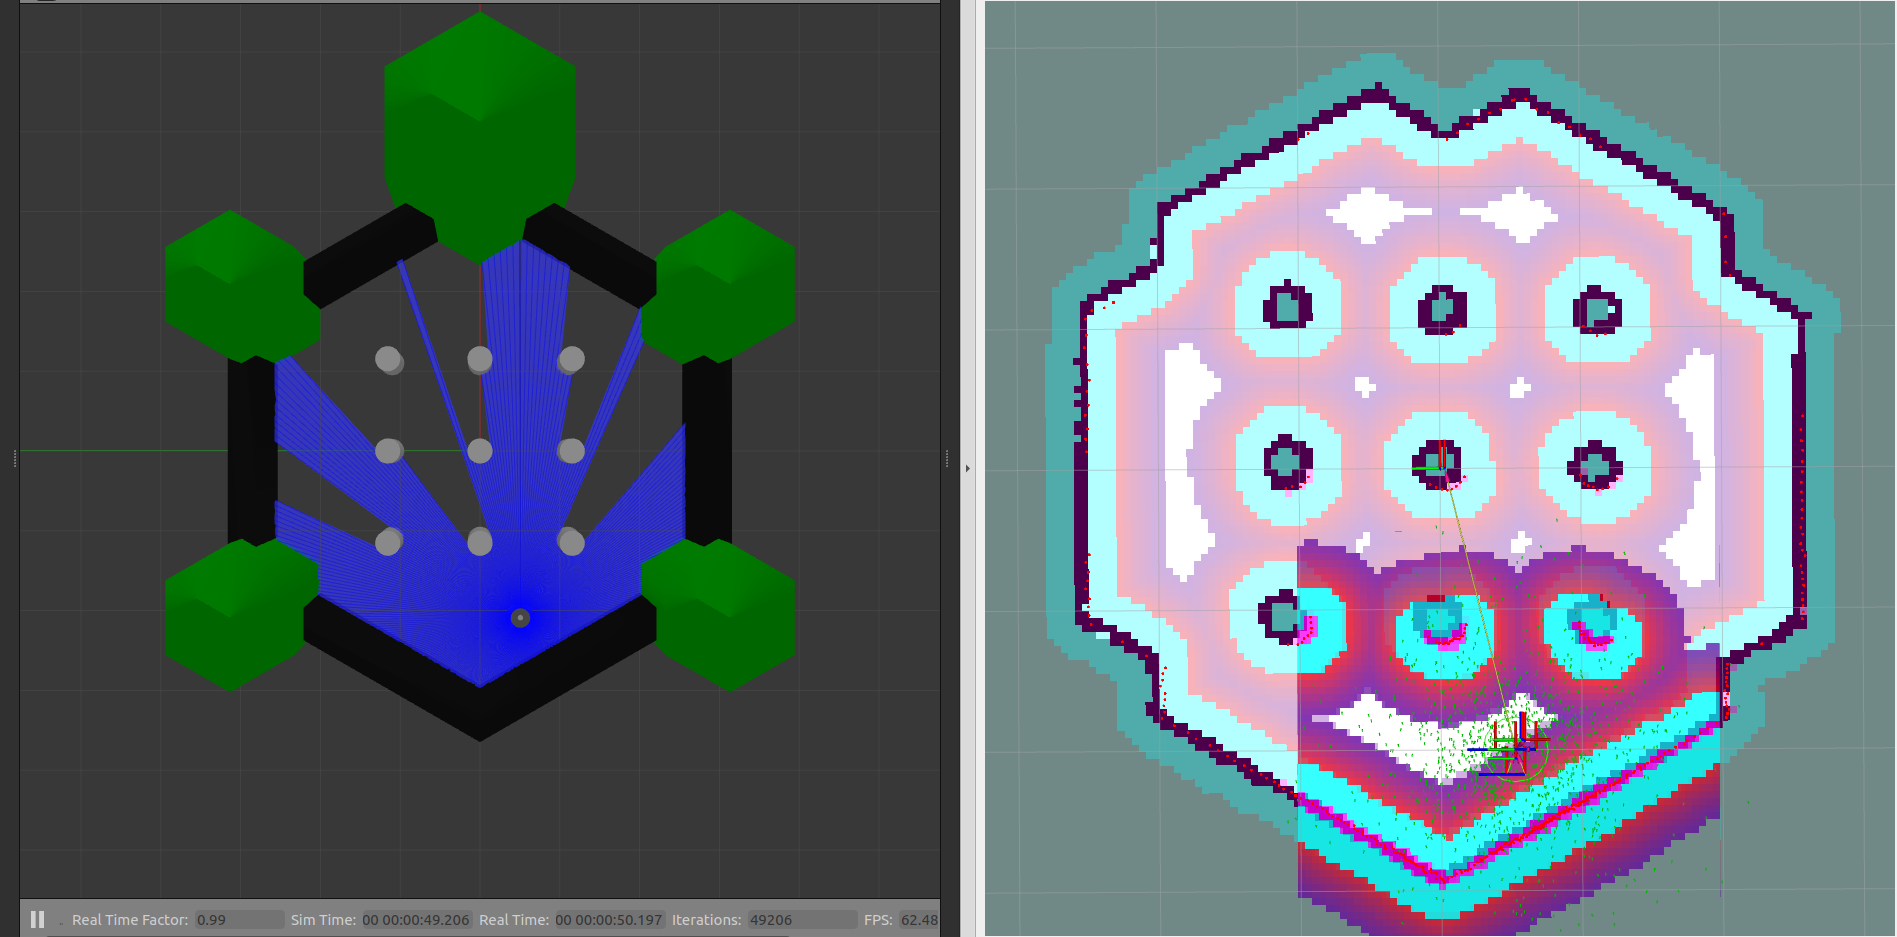
\includegraphics[width=\textwidth]{figures/screenshot_sim_world.png}
    \caption[Simulation environment]{Screenshot of Turtlebot3 in Gazebo (left) and RViz2 (right).}
    \label{fig:screenshot_simworld}
\end{figure}

Using Turtlebot3 means that we have no AGV forklift and, therefore, no direct implementation of the fork and its pick-and-place actions. Instead, these actions are simulated with behaviour tree nodes, as explained in Section \ref{ssec:custom_behavior_tree_nodes}. Lastly, the environment is simulated as a warehouse. A warehouse usually consists of shelves for pallets and goods, one or several loading docks, and charging stations for electric forklifts and/or AGVs. Our environment simulates such zones by passing coordinates of a hypothetical charging station, unload zone and four shelves to SemReBot2. 

\begin{figure}
    \centering
    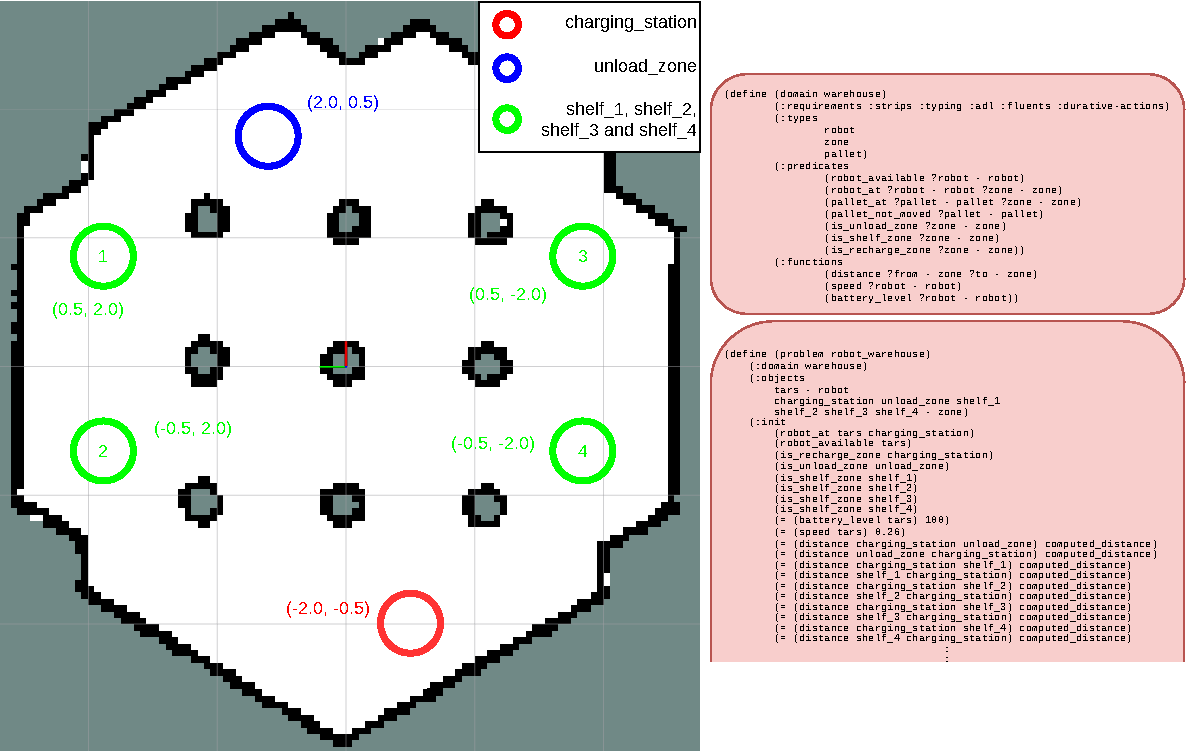
\includegraphics[width=0.8\textwidth]{figures/combined_domain.pdf}
    \caption[Simulated world knowledge]{A map of the different zones with correpsonding 2D coordinates (left) and domain and problem knowledge fed to SemReBot2 and PlanSys2 (right).}
    \label{fig:sim_world_knowledge}
\end{figure}

Turtlebot3 uses simulated LiDAR and odometry data for navigation, but neither SemReBot2 nor PlanSys2 receives data from sensors. Instead, they receive information about the physical/simulated world from a provided \verb|domain.pddl| file and voice commands processed by Whisper node and Mistral node. In addition, Task controller node's constructor is passing constant initial knowledge to PlanSys2, such as robot and zones instances and function values like battery level and distance between the zones. Sensor data is handled by Nav2, receiving waypoints to navigate to and goal poses from the Navigate BT node, which again is ticked by the Executor in PlanSys2.

For detailed information on plugins used in Nav2 and Gazebo, see Appendix \textcolor{red}{X}.

\section{Detailed}
This section will provide a detailed example of how SemReBot2 works in conjunction with PlanSys2, Nav2, and Turtlebot3. We provide an example at each step so the reader can follow along how speech is converted to robot actions. It can be divided into several steps.

\begin{figure}
    \centering
    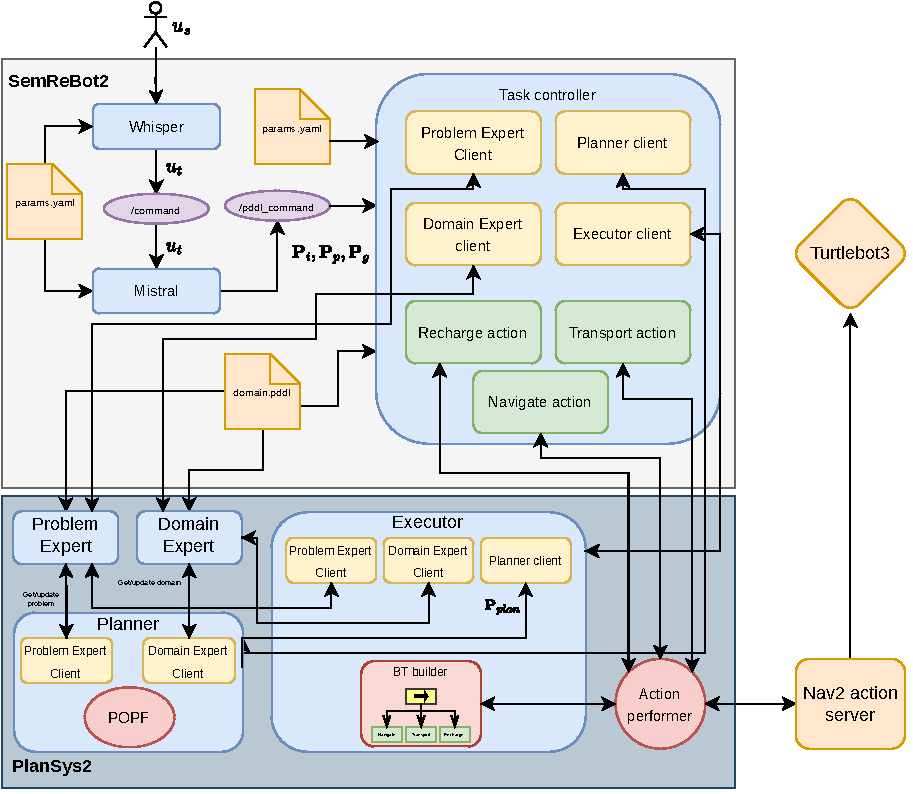
\includegraphics[width=0.8\textwidth]{figures/semrebot2.pdf}
    \caption[SemReBot2 detailed overview]{Detailed overview of data flow in SemReBot2 and PlanSys2 with Nav2 and Turtlebot3}
    \label{fig:semrebot2}
\end{figure}

\subsection{Step 1 - Speech-to-text}
When SemReBot2 is activated and a human is speaking, the audio stream $u_{s}$ is recorded mono with a sample rate of 16 kHz and 512 frames per buffer. The frames are concatinated to a single bytes object before its passed to Whisper as a \verb|NumPy| array of 16-bit integers. To decrease the inference time on Whisper, we transcribe $u_{s}$ with a chunk length of 30 seconds and a batch size of 24 chunks.

The first part of SemReBot2 can therefore be seen as a function that converts an audio signal into a sequence of words

\begin{equation}
    \label{eq:whisper_function}
    u_{t}=f(u_{s})
\end{equation}

\begin{example}\label{ex:whisper}
    Given the warehouse environment in Figure \ref{fig:sim_world_knowledge}, our robot TARS, an AGV forklift, is placed besides shelf 1 with 50\% battery capacity. A worker gives the command by voice

    \textit{TARS, move pallet number 1 from the unload zone to shelf number 1, and relocate pallet number 2 from the unload zone to shelf number 4.}

    SemReBot2 will recognise its being talked to and the command will be transcribed by Whisper, and published to the \verb|/command| topic.
\end{example}

\subsection{Step 2 - Create instances, predicates and goals}
Mistral receives the transcribed text $u_{t}$ and analyzes the semantics. Given the generated knowledge, system prompt and few-shot prompts, Mistral has learned how to output the correct instances, predicates and goals. They will be formatted into a single string and published to the \verb|/pddl_command| topic for further computation.

\begin{example}\label{ex:mistral}
    Continuing from Example \ref{ex:whisper}, Mistral extracts the necessary instances, predicates and goals from $u_{t}$ in the same format as defined in \verb|domain.pddl|:

    \begin{equation}
        \mathbf{P}_{i}=
        \begin{pmatrix}
            \text{p}_{1} \text{ pallet} \\
            \text{p}_{2} \text{ pallet}
        \end{pmatrix}
    \end{equation}
    
    \begin{equation}
        \mathbf{P}_{p}=
        \begin{pmatrix}
            \text{pallet\_at p}_{1} \text{ unload\_zone} \\    
            \text{pallet\_at p}_{2} \text{ unload\_zone} \\
            \text{pallet\_not\_moved p}_{1} \\
            \text{pallet\_not\_moved p}_{2}
        \end{pmatrix}
    \end{equation}

    \begin{equation}
        \mathbf{P}_{g} =
        \begin{pmatrix}
            \text{pallet\_at p}_{1} \text{ shelf\_1} \\
            \text{pallet\_at p}_{2} \text{ shelf\_4}
        \end{pmatrix}
    \end{equation}

Note that the predicates \verb|robot_at| and \verb|robot_available| is not used by Mistral due to the generated knowledge.
\end{example}

\subsection{Step 3 - Generate a PDDL plan}
The third step in SemReBot2 involves activating PlanSys2. The Task controller receives the instances, predicates and goals from Mistral, checks if they are eligible based on \verb|domain.pddl|, and passes them to the \verb|Planner|, \verb|Executor|, \verb|Problem Expert| and \verb|Domain Expert| through service calls.

\begin{example}\label{ex:task_controller}
    Continuing from Example \ref{ex:mistral}, the Task controller parses $\mathbf{P}_{i}$, $\mathbf{P}_{p}$ and $\mathbf{P}_{g}$ and make service calls to the \verb|Problem Expert| which adds the new knowledge to the \verb|problem.pddl| file.

    \begin{lstlisting}[caption={Parts of the problem file available for POPF. Only showing the added objects and initial knowledge received from Task controller.}, label=lst:ex_problem.pddl]
        (:objects
                :
            p1 p2 - pallet)
        (:init
                :
                :
            (pallet_at p1 unload_zone)
            (pallet_at p2 unload_zone)
            (pallet_not_moved p1)
            (pallet_not_moved p2))
        (:goal (and
            (pallet_at p1 shelf_1)
            (pallet_at p2 shelf_4)))
    \end{lstlisting}

    The \verb|Planner| receives the domain and problem file from the \verb|Problem Expert| and \newline\verb|Domain Expert| and makes a call to the POPF plugin, which generates the following plan:

    \begin{verbatim}
        0:      (navigate tars shelf_1 charging_station)      [13.598]
        13.599:	(recharge tars charging_station)              [10]
        23.6:   (navigate tars charging_station unload_zone)  [15.858]
        39.459: (transport tars pallet_1 unload_zone shelf_1) [8.159]
        47.619: (navigate tars shelf_1 unload_zone)           [8.159]
        55.779: (transport tars pallet_2 unload_zone shelf_4) [11.213]
    \end{verbatim}

    The plan shows all the PDDL actions necessary for TARS to complete the command from the worker. The left column shows the amount of time passed, the middle column shows the PDDL action with necessary parameters, and the third column shows the time it takes to complete the action. The time it takes to complete an action is based on the robot's speed and distance from one pose to another, computed dynamically. Note that the second PDDL action is to recharge the robot, as TARS, in our example, begins with 50\% battery capacity.
    
\end{example}

\subsection{Step 4 - Building a behaviour tree and executing actions}
Once the \verb|Executor| receives the plan from the \verb|Planner|, it converts the plan to a BT, see Figure \textcolor{red}{bilde av BT builder}, and an execution graph that defines the execution order of the actions. The order of actions is defined by the time computed by POPF.

\begin{example}\label{ex:bt_builder}
    A suitable BT from the PDDL plan in Example \ref{ex:task_controller} can be seen in Figure \ref{fig:example_bt}. All of the custom BT nodes are sequence nodes.

    \begin{figure}[ht]
        \centering
        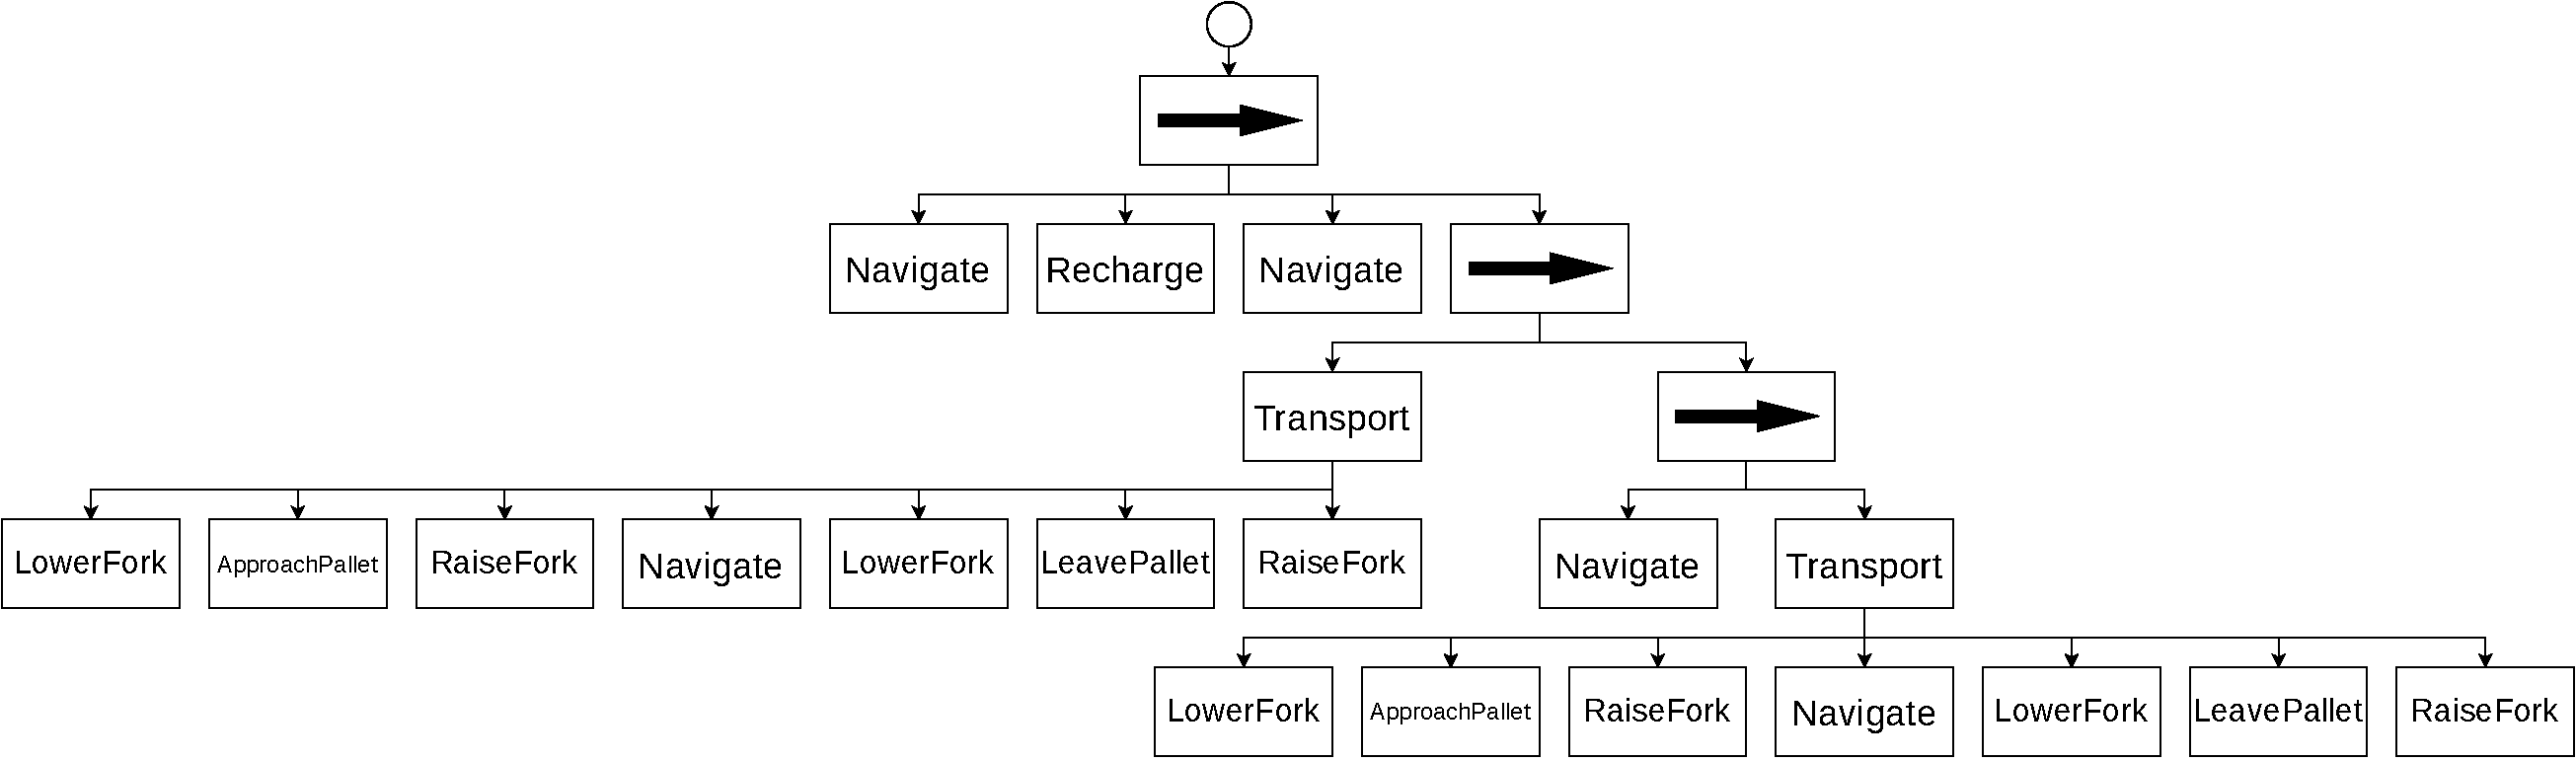
\includegraphics[width=\textwidth]{figures/example_bt.pdf}
        \caption[BT from SemReBot2 example]{A suitable BT for the plan generated in Example \ref{ex:task_controller}.}
        \label{fig:example_bt}
    \end{figure}
\end{example}

PlanSys2's action performer will tick the BT. Once the \verb|Navigate| BT node is ticked, it will make a call to Nav2's \verb|NavigateToPose| action server which then makes TARS move to the goal pose in the \verb|navigate| PDDL action.

Files \verb|domain.pddl| and \verb|problem.pddl| can be seen in Appendix \textcolor{red}{X}.

\section{Hardware requirements}
SemReBot2 is designed to run locally on a single GPU. We run it on a GPU with 12 GB memory, which is more than enough when loading Whisper Large with flash attention and Mistral 7B Instruct in 4-bit quantized size.
\chapter{Experiments and Results}\label{ch:experiments}
This section will present the experiments carried out in the different parts of SemReBot2 as well as a full system test. For a discussion around the results, see Section \ref{ch:discussion}. The experiments aim to highlight the advantages and disadvantages of the different model sizes, and each subsection will present the key findings for each part of SemReBot2. A full description of the test sets and results can be found in Appendix \textcolor{red}{X}. 

The experiments are primarily targeted at the specific use case of SemReBot2. Creators of models and packages used in SemReBot2 have conducted their own experiments for general purpose use, and the reader is encouraged to read the official papers of Whisper\cite{radford_robust_2022}, Mistral\cite{jiang_mistral_2023}, POPF\cite{coles_forward-chaining_2021} and PlanSys2\cite{martin_plansys2_2021} respectively for general performance experiment results.

\section{Whisper}\label{sec:Whisper_experiments}
The experiments conducted on Whisper were performed to compare the performance of different model sizes and to determine whether loading models with flash attention increased or decreased performance. The chosen metrics were WER, RTF, allocated memory during inference, and inference time.

The test set consists of ten audio files with a corresponding reference text. The audio files are news segments with a duration of 123 seconds to 824 seconds downloaded from Rev.com\cite{revcom_transcript_2024}, accompanied by a transcribed text.

The key results can be seen in Figure \ref{fig:whisper_avg}.

\begin{figure}[ht]
    \centering
    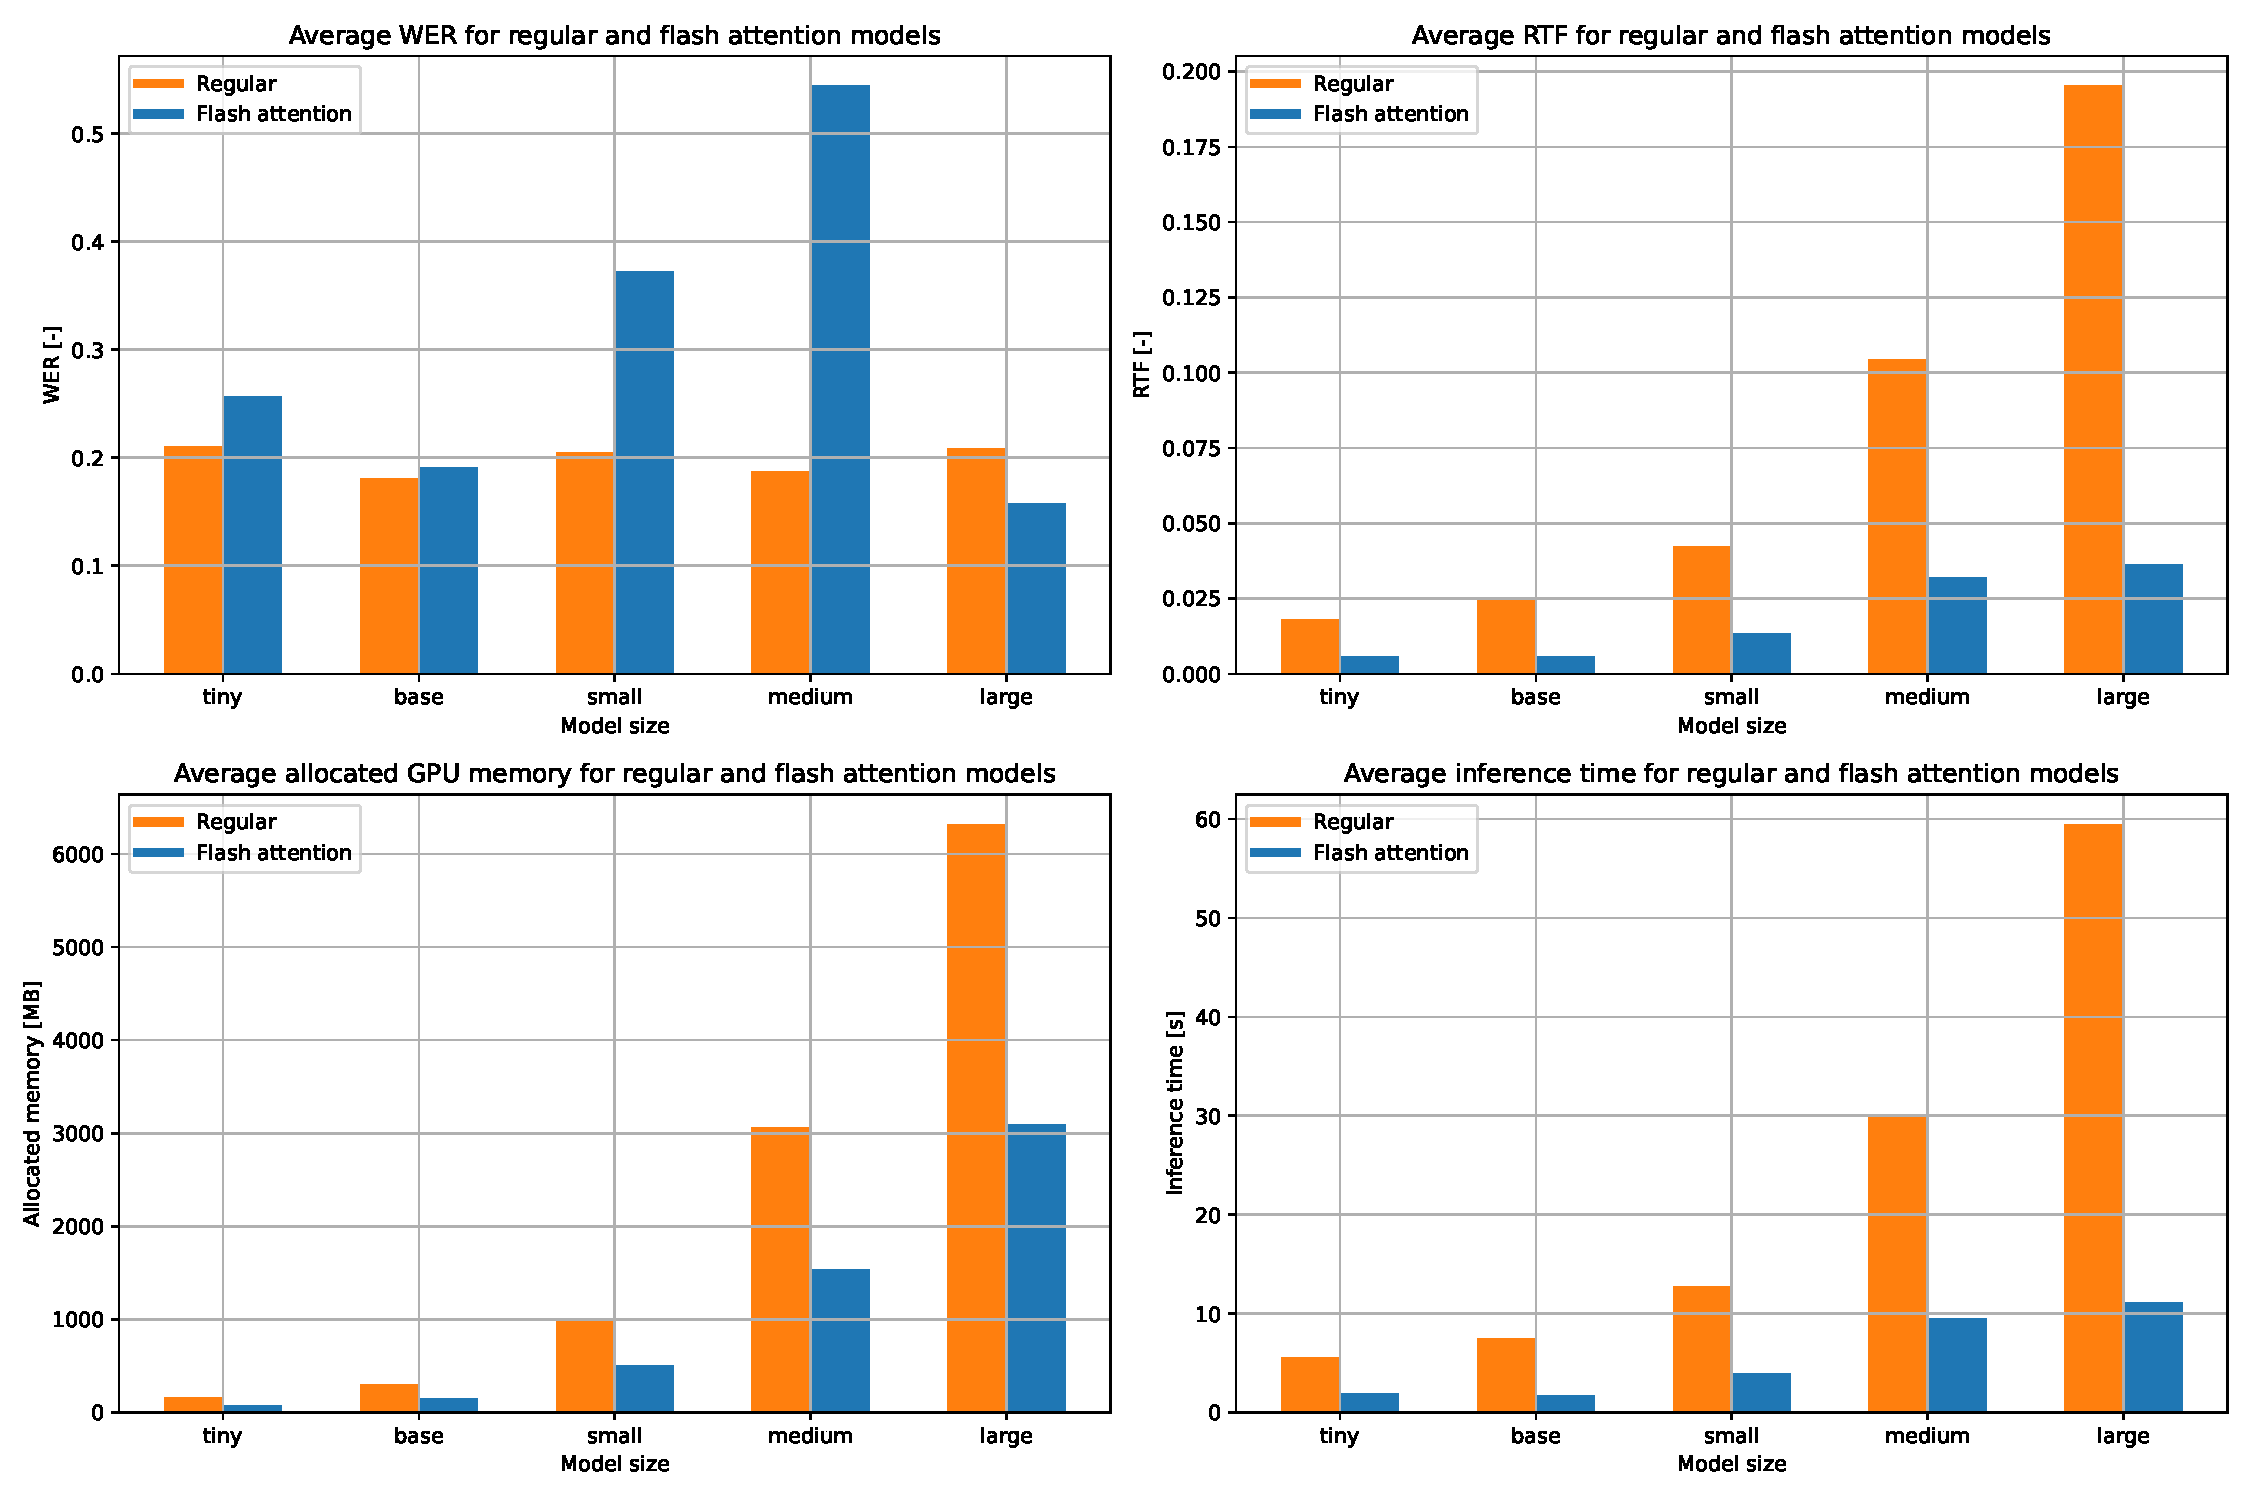
\includegraphics[width=\textwidth]{figures/avg.pdf}
    \caption[Whisper experiment results]{Comparison of Whisper model sizes loaded with flash attention and not. Measured metrics are WER (top left), RTF (top right), allocated memory during inference (bottom left) and average inference time (bottom right).}
    \label{fig:whisper_avg}
\end{figure}

\section{Mistral}\label{sec:Mistral_experiments}
Experiments conducted on Mistral were specific to the PDDL domain and the desired output format used in SemReBot2. We created two test sets where Mistral was given a PDDL domain with types and predicates available, as well as a natural language command.

\subsection{Test sets}
In test set 1, containing ten elements, each element consists of a domain extracted from the Github repository \verb|pddl-generators| by AI-Planning community\cite{favorito_ai-planningpddl-generators_2024}\footnote{This repository contain domains and problems used to generate benchmarks for the International Planning Competition.}. We then accompany each domain with a natural language command and a solution containing the correct instances, predicates, and goals in the correct format as SemReBot2 expects. An element of test set 1 can be seen in Listing \ref{lst:elem_test_set_1}

In test set 2, all eleven elements contain the same PDDL domain, which is the same domain as in the simulated environment, but different accompanying natural language commands and solutions. This test set is specific to the SemReBot2 use case.

\begin{lstlisting}[caption={An element of test set 1 showing the domain and command Mistral is given. The output is to measure if Mistral is correct or wrong.}, label=lst:elem_test_set_1]
{
"domain":"(:types worker task location)
          (:predicates (available ?worker - worker)
          (assigned ?task - task ?worker - worker)
          (located ?task - task ?location - location)
          (completed ?task - task))",
"command":"Assign the new tasks to workers efficiently. Task1 is at
           Location1, Task2 at Location2.
           Worker1 starts available.",
"solution":"instance worker1 worker|instance task1 task|
            instance task2 task|instance location1 location|
            instance location2 location|predicate available worker1|
            predicate located task1 location1|
            predicate located task2 location2|
            goal assigned task1 worker1|goal assigned task2 worker1|"
},
           
\end{lstlisting}

\subsection{Shot sets}
For each test set, we created one or two sets that we call "shot sets".

For test set 1, we created two shot sets, shot set 1 and shot set 2, with PDDL domains from \verb|pddl-generators| (but not the same as in test set 1), containing 32 elements with an accompanying natural language command and an output. The difference between shot set 1 and shot set 2 is that shot set 1 is unlabelled, while shot set 2 is labelled. That is, all the outputs in shot set 1 are correct, while every other output in shot set 2 is correct or wrong. So, shot set 2 contains an extra marker \verb|label| which is either \verb|correct| or \verb|wrong|. An element of shot set 2 can be seen in Listing \ref{lst:elem_shot_set_2}.

For test set 2, we used the same shot set as test set. However, if Mistral was running a test on element \verb|i| in test set 2, the shot set would contain all the previous elements in test set 2 as shots. This means that shot set 3 contain ten elements (\verb|len(test_set_2) - 1|).

\begin{lstlisting}[caption={An element of shot set 2. Notice the "label" marker. The output is wrong due to the text before first instance.}, label=lst:elem_shot_set_2]
{
"domain": "(:types portable location)
           (:predicates (at ?y - portable ?x - location)
           (in ?x - portable) (is-at ?x - location)) ",
"input":"Transport all the four objects to their respective location:
         first object to location 3, second object to location 0,
         third object to location 1 and fourth object at location 2.
         Also, go to location 1 afterwards. The four objects are now
         at location 3, location 1, location 2 and location 0
         respectively. We are in location 4.",
"output":"Here are the instances, predicates and goals:
          instance l0 location|instance l1 location|
          instance l2 location|instance l3 location|
          instance l4 location|instance o0 portable|
          instance o1 portable|instance o2 portable|
          instance o3 portable|predicate at o0 l3|
          predicate at o1 l1|predicate at o2 l2|predicate at o3 l0|
          predicate is-at l4|goal at o0 l3|goal at o1 l0|
          goal at o2 l1|goal at o3 l2|goal is-at l1|",
"label":"wrong"
},
\end{lstlisting}

\subsection{System prompts}\label{ssec:system_prompt}
For all the tests that we ran, we created three different system prompts. A system prompt represents a chat history between a user and the assistant (read Mistral). All three system prompts explain what role Mistral has, its goal, and show one example of domain, natural language command, and expected output. The difference between the three is the length and the amount of detail Mistral is given. The prompts range between what we call "short and precise", "medium detailed", and "long and detailed". Listing \ref{lst:mistral_system_prompt} shows the short and precise system prompt.

\begin{lstlisting}[caption={The short and precise system prompt. domains[0], inputs[0] and outputs[0] is the first element from the shot set.}, label=lst:mistral_system_prompt]
system_prompt = """

As a PDDL assistant, your task is to outline the available instances,
predicates, and goals based on the provided domain and command.
Answer in the format shown after ### Output ###.

"""

message = [

{'role': 'user', 'content': system_prompt + f' Here is a domain:
                            {domains[0]}, and command {inputs[0]}.
                            ### Output ### {outputs[0]}.'},
                            
{'role': 'assistant', 'content': 'Understood.
                            Awaiting new domain and command.'},
                            
],
\end{lstlisting}

\subsection{Tests}
The first test was performed to see performance differences between a fine-tuned model for "SemReBot2 use" and zero-, one-, and few-shot prompting.

\subsection{Fine-tuned model}

\subsection{Pre-prompted model}
For the pre-prompted model tests, we ran three different tests:

\begin{itemize}
    \item Generic PDDL domain without labels
    \item Generic PDDL domain with labels
    \item Specific PDDL domain without labels
\end{itemize}

Every test was set up the same way: We first load the model into memory, extract one element from the test set, extract zero or more elements from the shot set depending on the number of iterations, run inference, and record the output before writing it to a file for storage. For all elements in a test set, we ran through all the elements in a shot set. This means that we recorded \verb|len(test_set)*len(shot_set)| number of test runs for each test set. We ensured that there was no information from previous test runs in Mistral by deleting and reloading the model before every inference run. See Appendix \textcolor{red}{X} for the model parameters used during the testing.

\begin{algorithm}\label{alg:mistral_test}
    \caption{Testing Mistral}
    \begin{algorithmic}[1]
        \State Load shot set, test set and system prompts
        \For{\textbf{each} test \textbf{in} test set}
            \For{\textbf{each} system prompt \textbf{in} system prompts}
                \For{\textbf{each} shot \textbf{in} shot set}
                    \State messages := system prompt + shot + test
                    \State Load model into memory
                    \State Perform model inference on messages
                    \State Write metric results to file
                    \State Delete model from memory and release resources
                \EndFor
            \EndFor
        \EndFor
    \end{algorithmic}
\end{algorithm}

In all tests, we measured inference time, allocated GPU memory during inference, model input size, and the output from Mistral compared to the solution. For the output, we defined four metrics: precision, recall,
F1 score and our own metric accuracy. Accuracy is computed by comparing the output instances, predicates and goals compared to the solution instances, predicates and goals. The evaluation metric is subdivided
into four distinct categories: $accuracy_{instances}$, $accuracy_{predicates}$, $accuracy_{goals}$ and $accuracy_{total}$.

\begin{equation}\label{eq:mistral_accuracy_metric}
    accuracy_{type}(\text{domain}, \text{command})=
    \begin{cases}
        1 & \text{if } output_{type} = solution_{type} \\
        0 & \text{otherwise}
    \end{cases}
\end{equation}

As seen in Equation \ref{eq:mistral_accuracy_metric}, each category, except for $accuracy_{total}$, employs a binary classification approach, in which the precision is deemed "correct" iff the output is exactly like the solution, disregarding variations in variable names. The total accuracy is then defined as

\begin{equation}\label{eq:mistral_total_accuracy_metric}
    accuracy_{total}=accuracy_{instances}\times accuracy_{predicates}\times accuracy_{goals}
\end{equation}

\subsubsection{Specific PDDL domain tests}
For the specific PDDL domain tests we evaluated Mistral's performance for three different prompts, with and without generated knowledge on test set 2. The generated knowledge was given as everything in the domain
that was true when Mistral is initiated.

\begin{lstlisting}[caption={The generated knowledge available to Mistral at every test run.}, label=lst:generated_knowledge]
    generated_knowledge = """
        instance tars robot|instance charging_station zone|instance unload_zone zone|instance shelf_1 zone|instance shelf_2 zone|instance shelf_3 zone|instance shelf_4 zone|
        predicate robot_availabletars|predicate is_recharge_zone charging_station|predicate is_unload_zone unload_zone|predicate is_shelf_zone shelf_1|predicate is_shelf_zone shelf_2|
        predicate is_shelf_zone shelf_3|predicate is_shelf_zone shelf_4|"""
\end{lstlisting}

The F1 score, inference time and allocated memory for the specific domain tests can be seen below.



\section{POPF}\label{sec:POPF_experiments}
We tested POPF isolated from SemReBot2 and PlanSys2 by giving it a \verb|domain.pddl| and different
\verb|problem.pddl| files. The domain and problems were solely relevant to SemReBot2's use case. We
checked 14 different scenarios one time each. As POPF is a deterministic AI planner, we only had to
check every scenario one time.

The scenarios ranged from simple navigation tasks only, to picking up one to 10 pallets and placing
them at different locations. We also checked the planners ability to plan for battery capacity,
logical errors in the problem file and its ability to plan the shortes possible path.

We created three different metrics, success rate, time and battery efficiency and planner time, where success
is a binary metric with "Yes/No" and time and battery efficiency is the ratio of the planners output
time and battery matched against an optimal answer created by us.

\begin{equation}\label{eq:popf_efficiency_metrics}
    0.00 \leq \eta_{time}, \eta_{battery} \leq 1.00
\end{equation}

The planner time is the time it takes for POPF to create a plan once it receives the domain and problem
file.

As with the simulation environment, the distance and time taken between waypoints is computed dynamically.


\section{SemReBot2 full system tests}\label{sec:SemReBot2_experiments}
\chapter{Discussion}\label{ch:discussion}

\begin{itemize}
    \item Local vs. cloud computing
    \item Only allow Mistral types and predicates from domain.pddl
    \item Keep AI use to minimum for safe application
    \item Prompt flags
    \item Why Gazebo, Turtlebot3 and Nav2 --> rclcpp::actions??
    \item I don't take into account the obstacles in Gazebo sim. Distances is computed with Eucledian distance. Also, no sensor data is feeded to SemReBot2, so the only info it knows is from voice and domain.pddl.
    \item Why PDDL and BT?
\end{itemize}
\chapter{Conclusion}



\printbibliography[title=References]

\appendix
\chapter{Name of Appendix}

\begin{itemize}
    \item AI model parameters
    \item Demo video
    \item Nav2 and Gazebo plugins
    \item domain.pddl, problem.pddl used in example
    \item Test sets and test results
    \item Mistral test model params
\end{itemize}

\section{Whisper experiment}

\begin{figure}
    \centering
    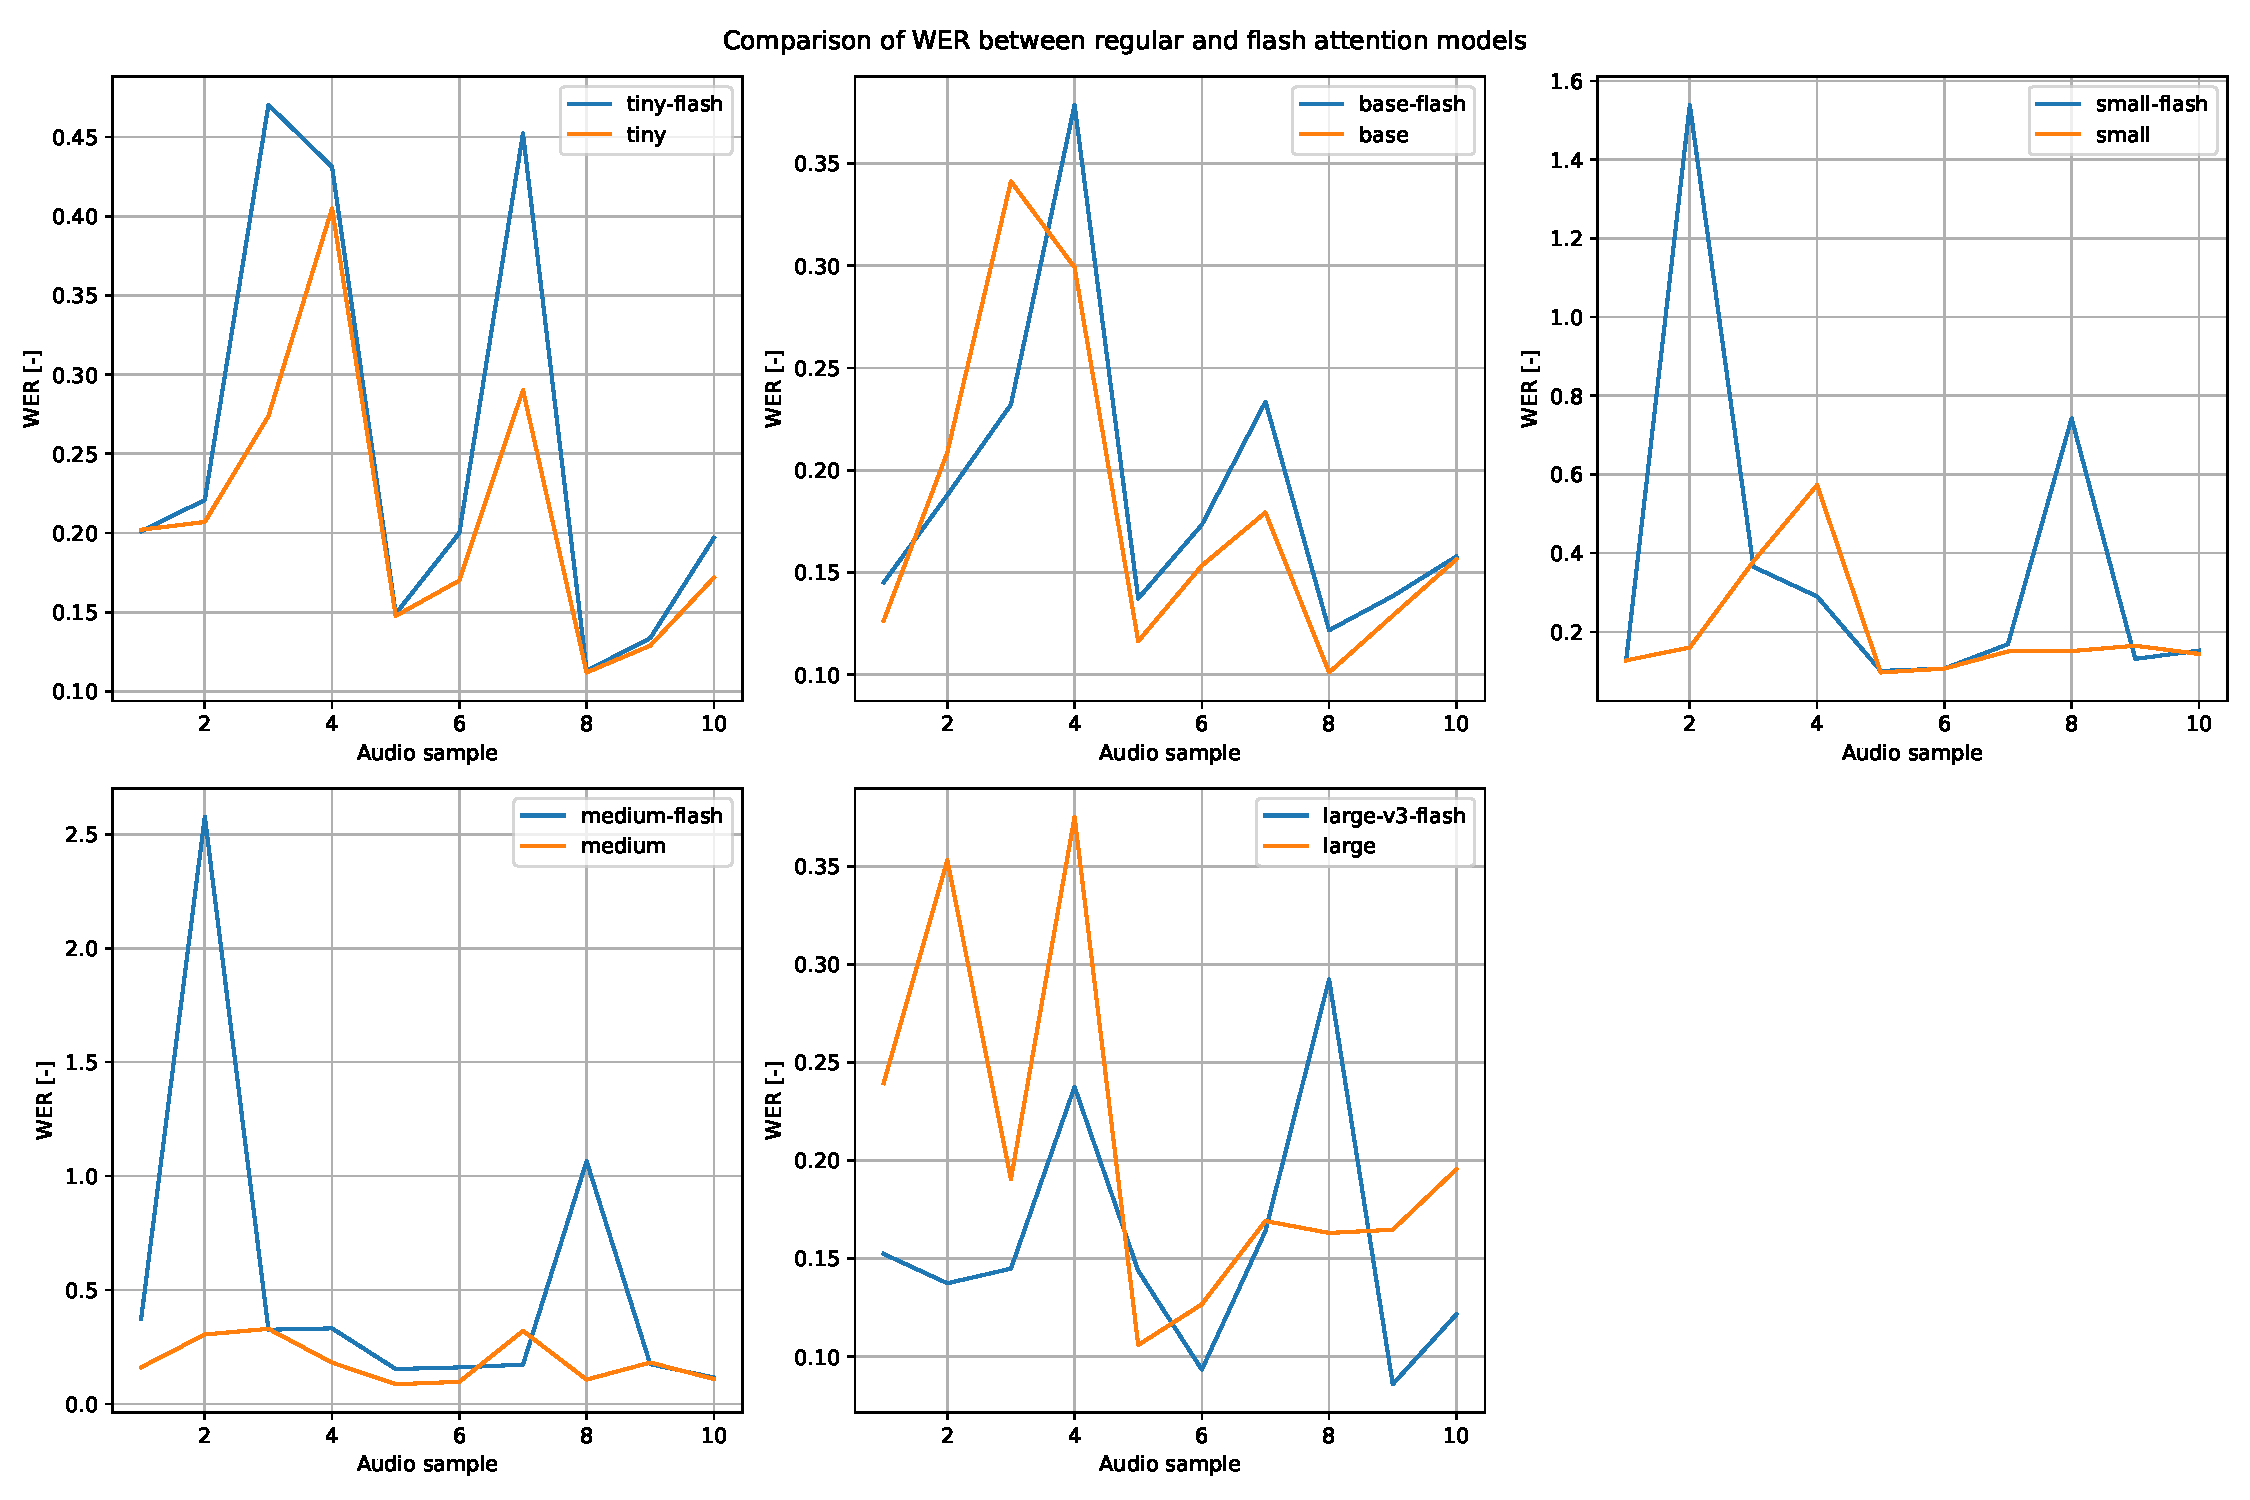
\includegraphics[width=\textwidth]{figures/wer.pdf}
    \caption{Caption}
    \label{fig:whisper_wer}
\end{figure}

\begin{figure}
    \centering
    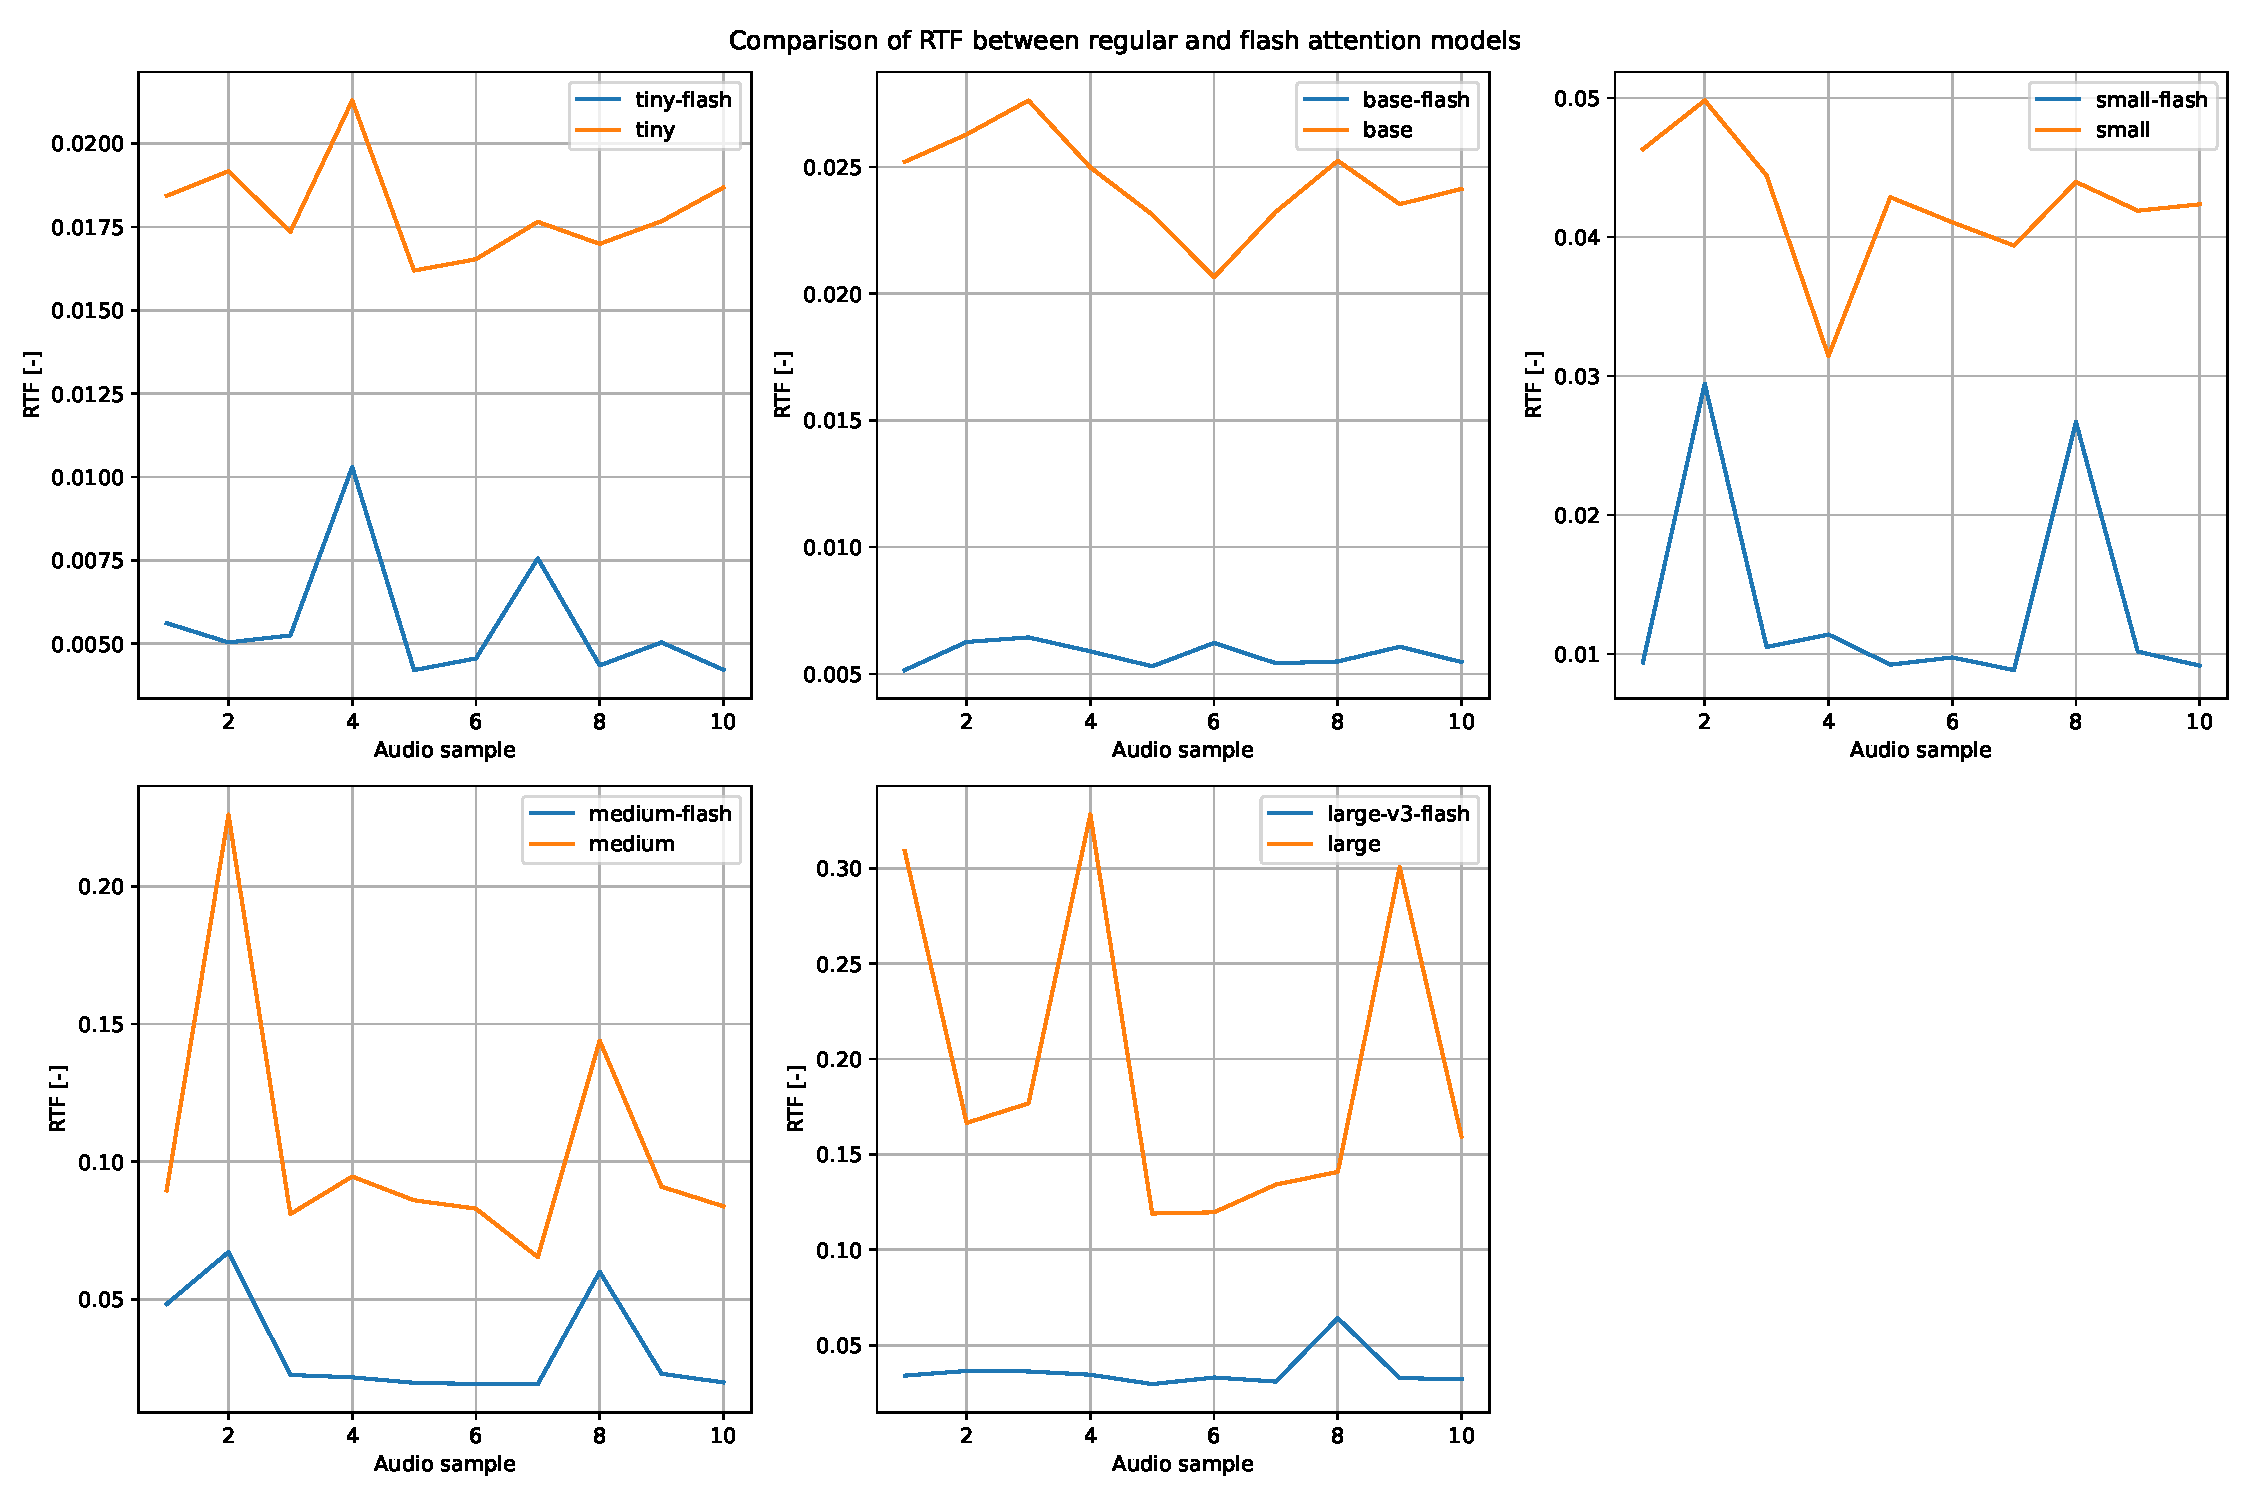
\includegraphics[width=\textwidth]{figures/rtf.pdf}
    \caption{Caption}
    \label{fig:whisper_rtf}
\end{figure}

\begin{figure}
    \centering
    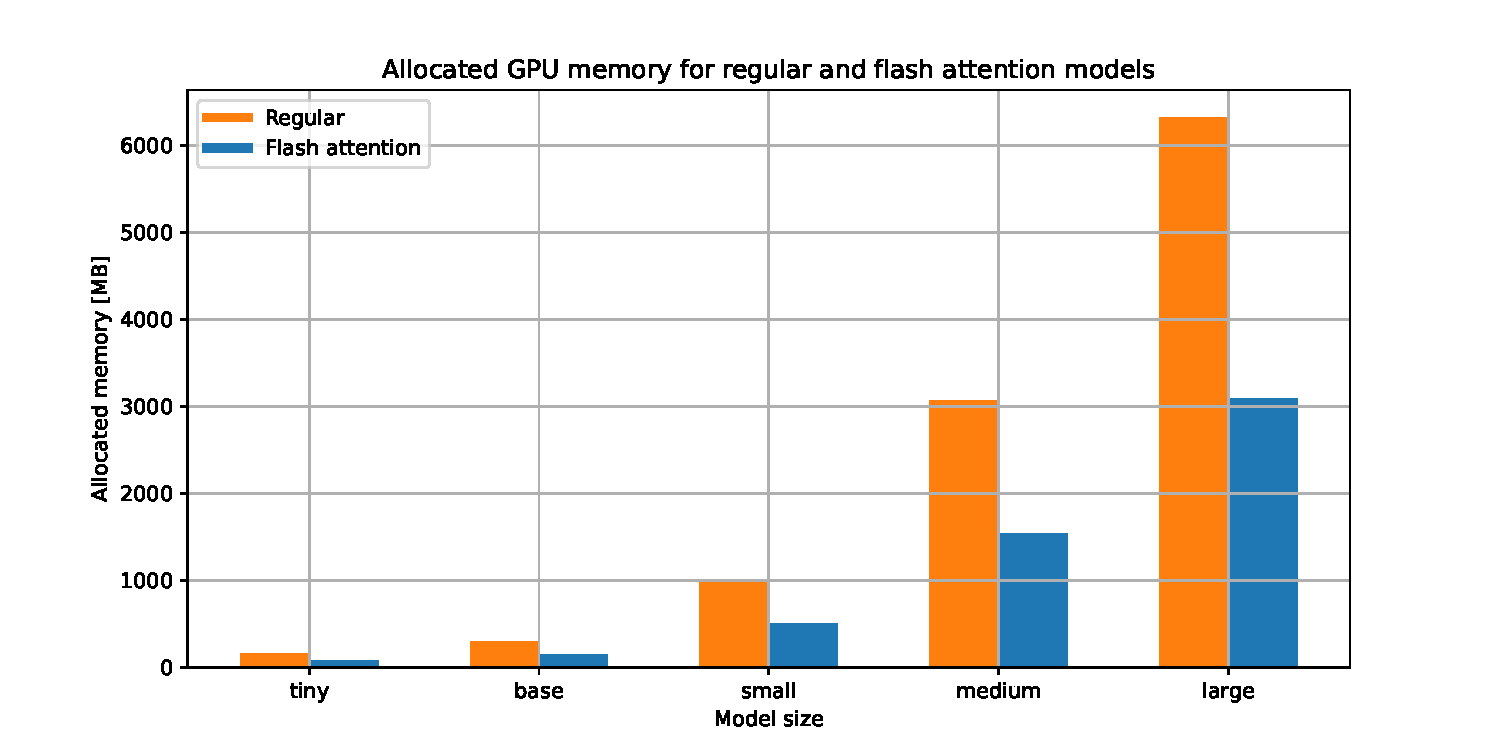
\includegraphics[width=\textwidth]{figures/memory.pdf}
    \caption{Caption}
    \label{fig:whisper_memory}
\end{figure}

\begin{figure}
    \centering
    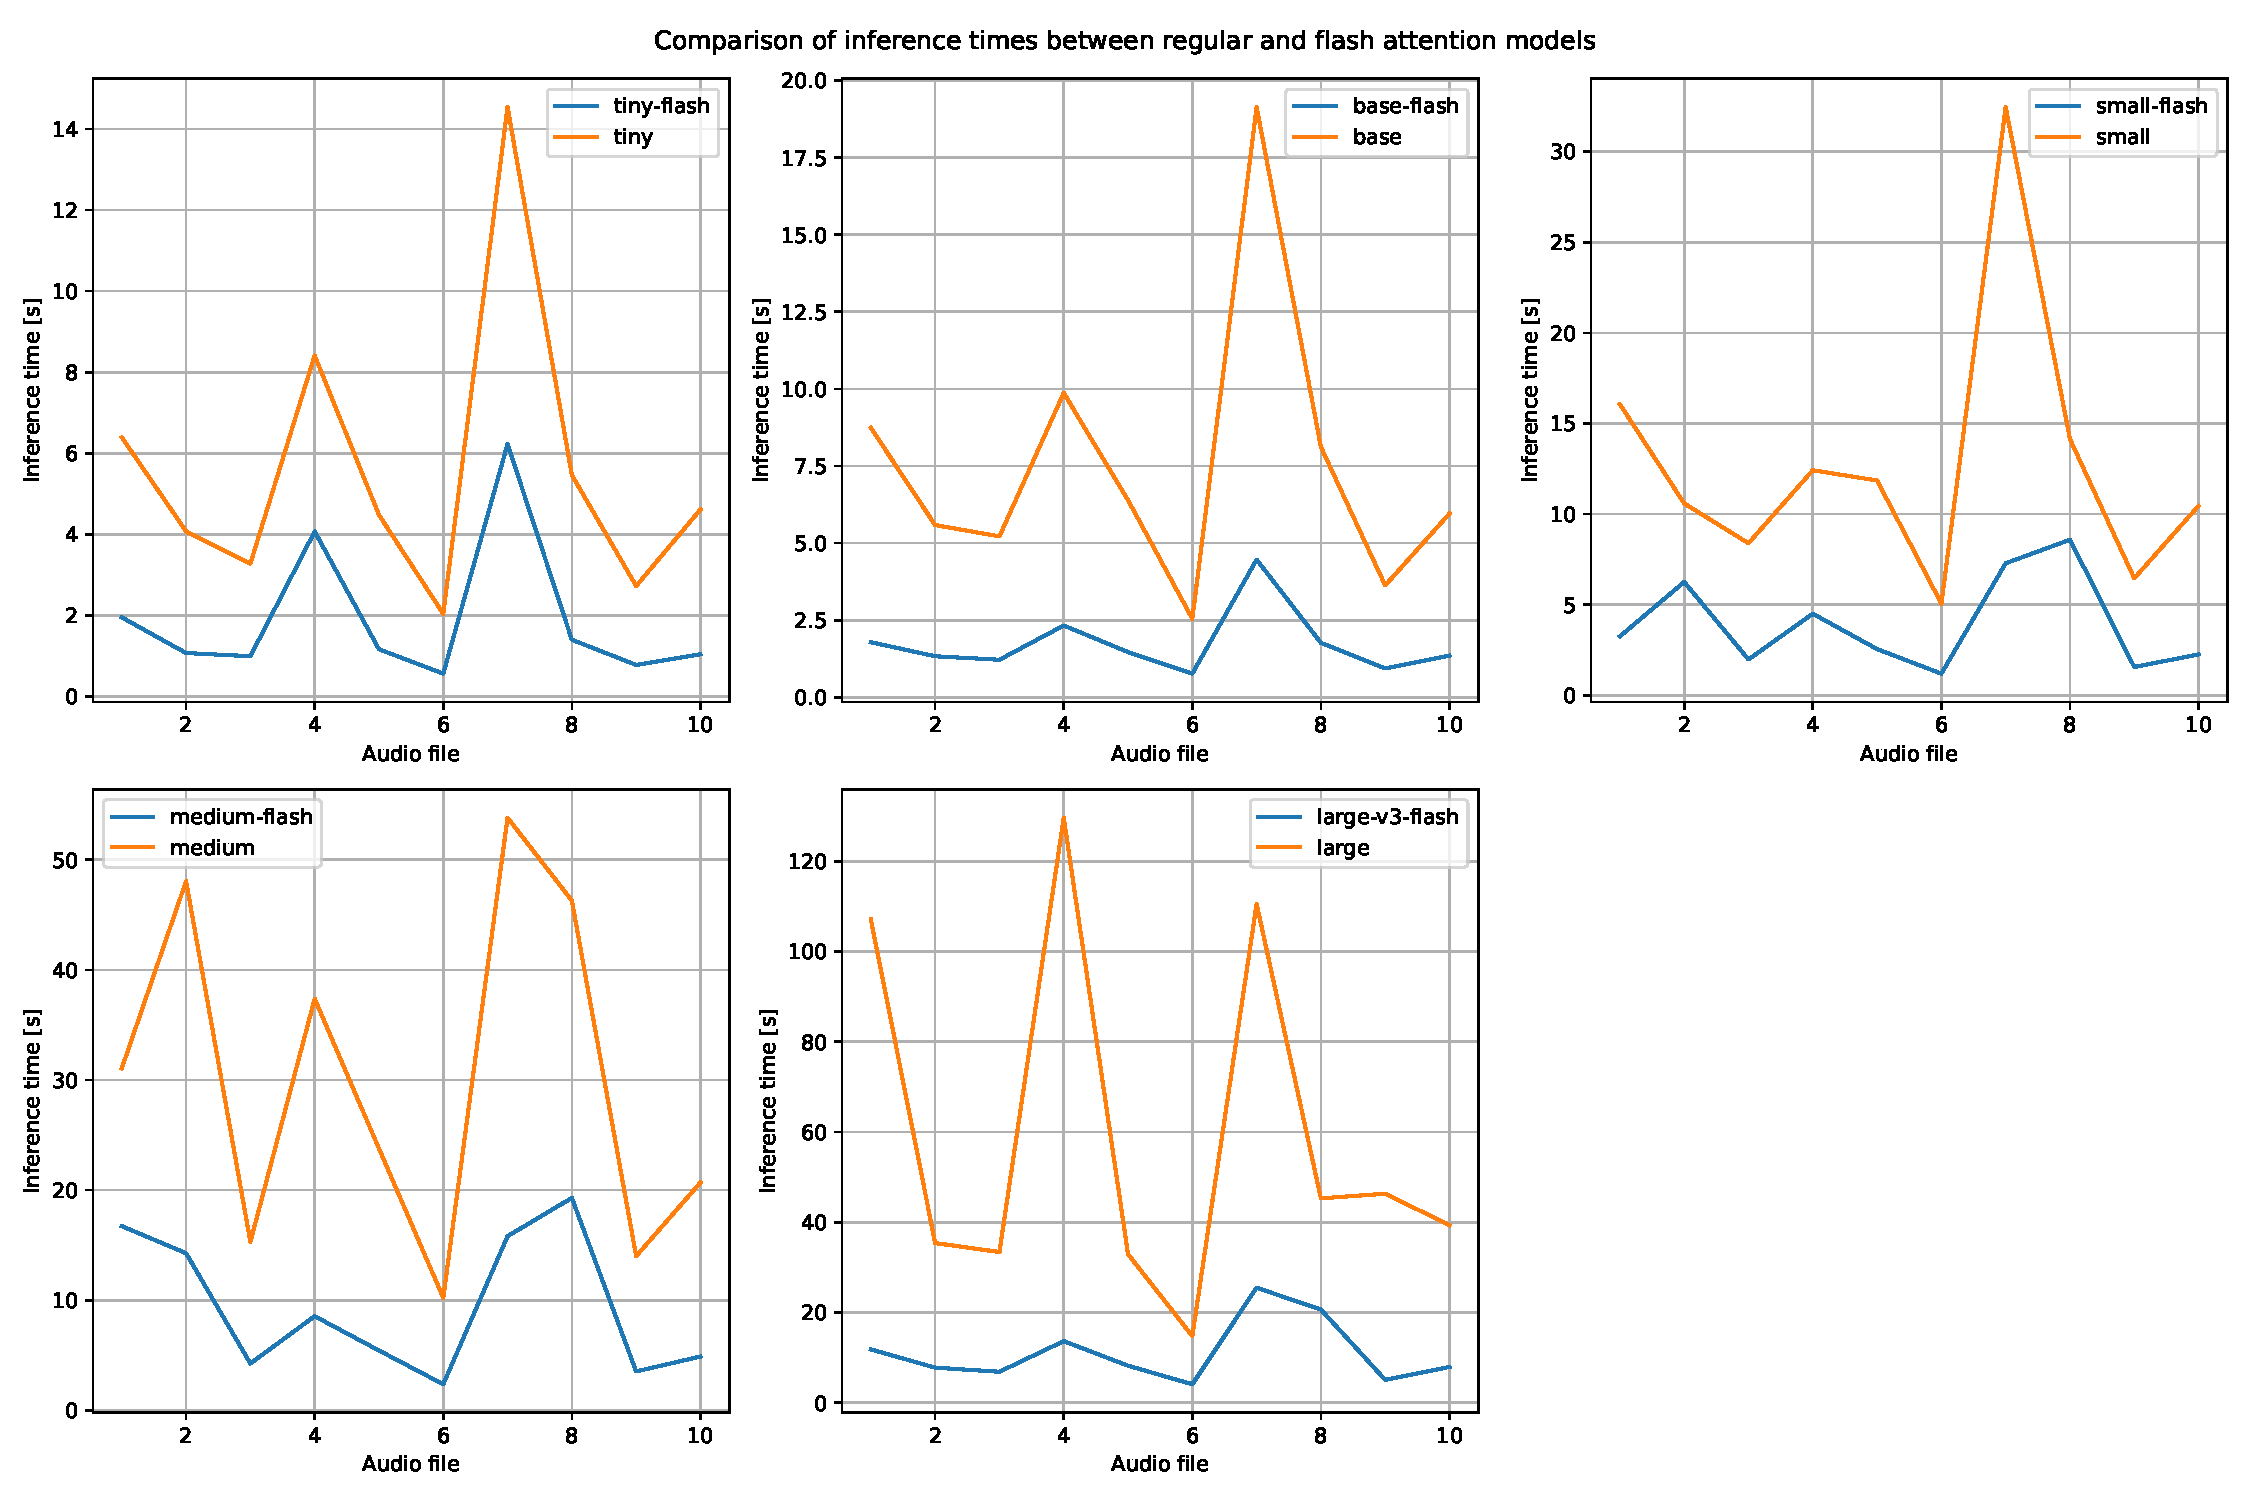
\includegraphics[width=\textwidth]{figures/inf_time.pdf}
    \caption{Caption}
    \label{fig:whisper_inf_time}
\end{figure}

\begin{figure}
    \centering
    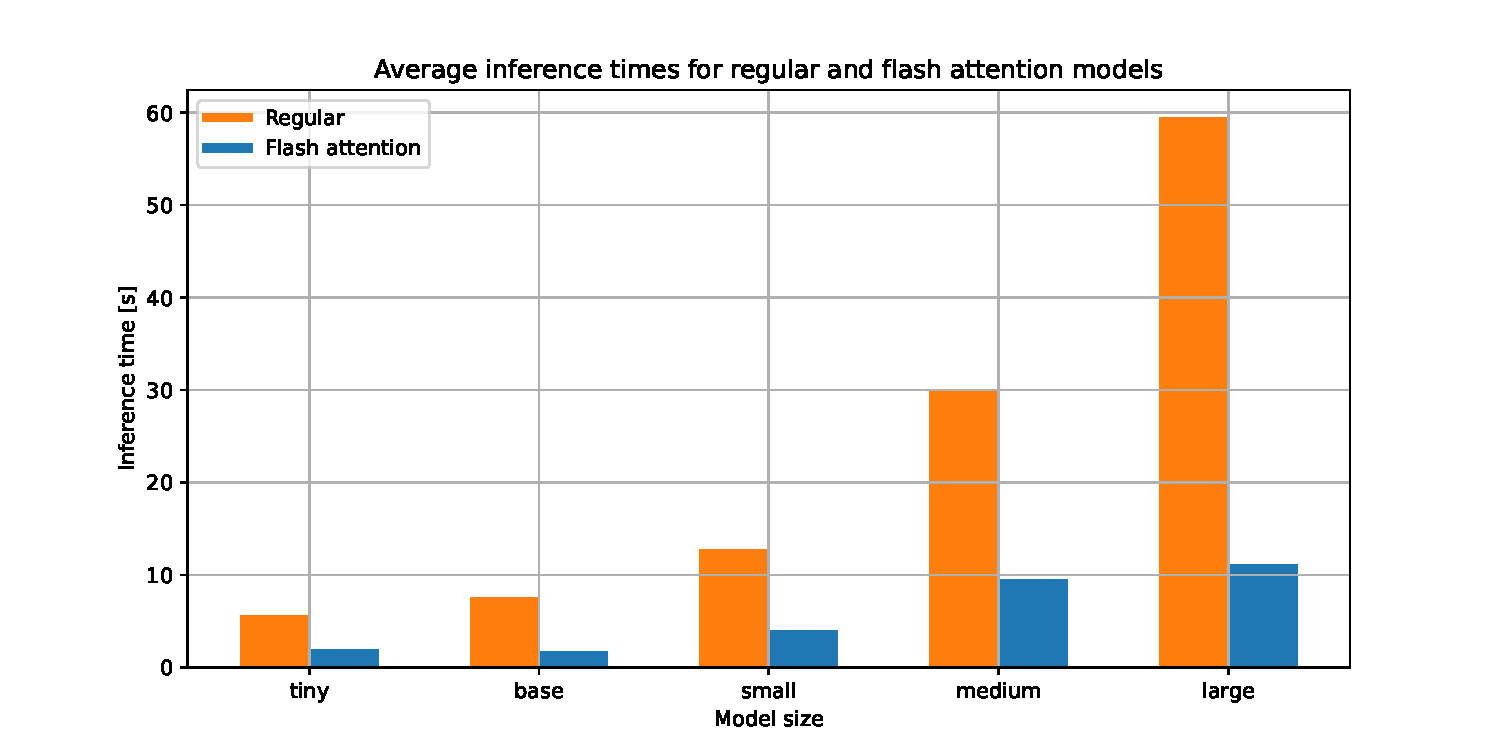
\includegraphics[width=\textwidth]{figures/avg_inf_time.pdf}
    \caption{Caption}
    \label{fig:whisper_avg_inf_time}
\end{figure}

\end{document}